\section{Zmiana świadczonych usług}

Zmiana świadczonych usług to ważna z punktu widzenia wykonawcy funkcjonalność. Zapewnia ograniczenie przydzielanych mu zleceń jedynie do tych, których realizacją może być zainteresowany. Rysunek \ref{fig:services} jest zrzutem ekranu, który ją prezentuje.
Sam wybór usług jest dokonywany poprzez zaznaczenie na liście. W celu lepszej organizacji i zwiększenia przejrzystości zostały one pogrupowane w kategorie, z których w danej chwili tylko jedna może być rozwinięta. Wymaga się, aby wykonawca świadczył przynajmniej jedną usługę. Jeżeli takowa nie jest określona, to wyświetlany jest komunikat mówiący o konieczności jej wybrania.

\begin{figure}[ht!]
  \centering
  \fbox{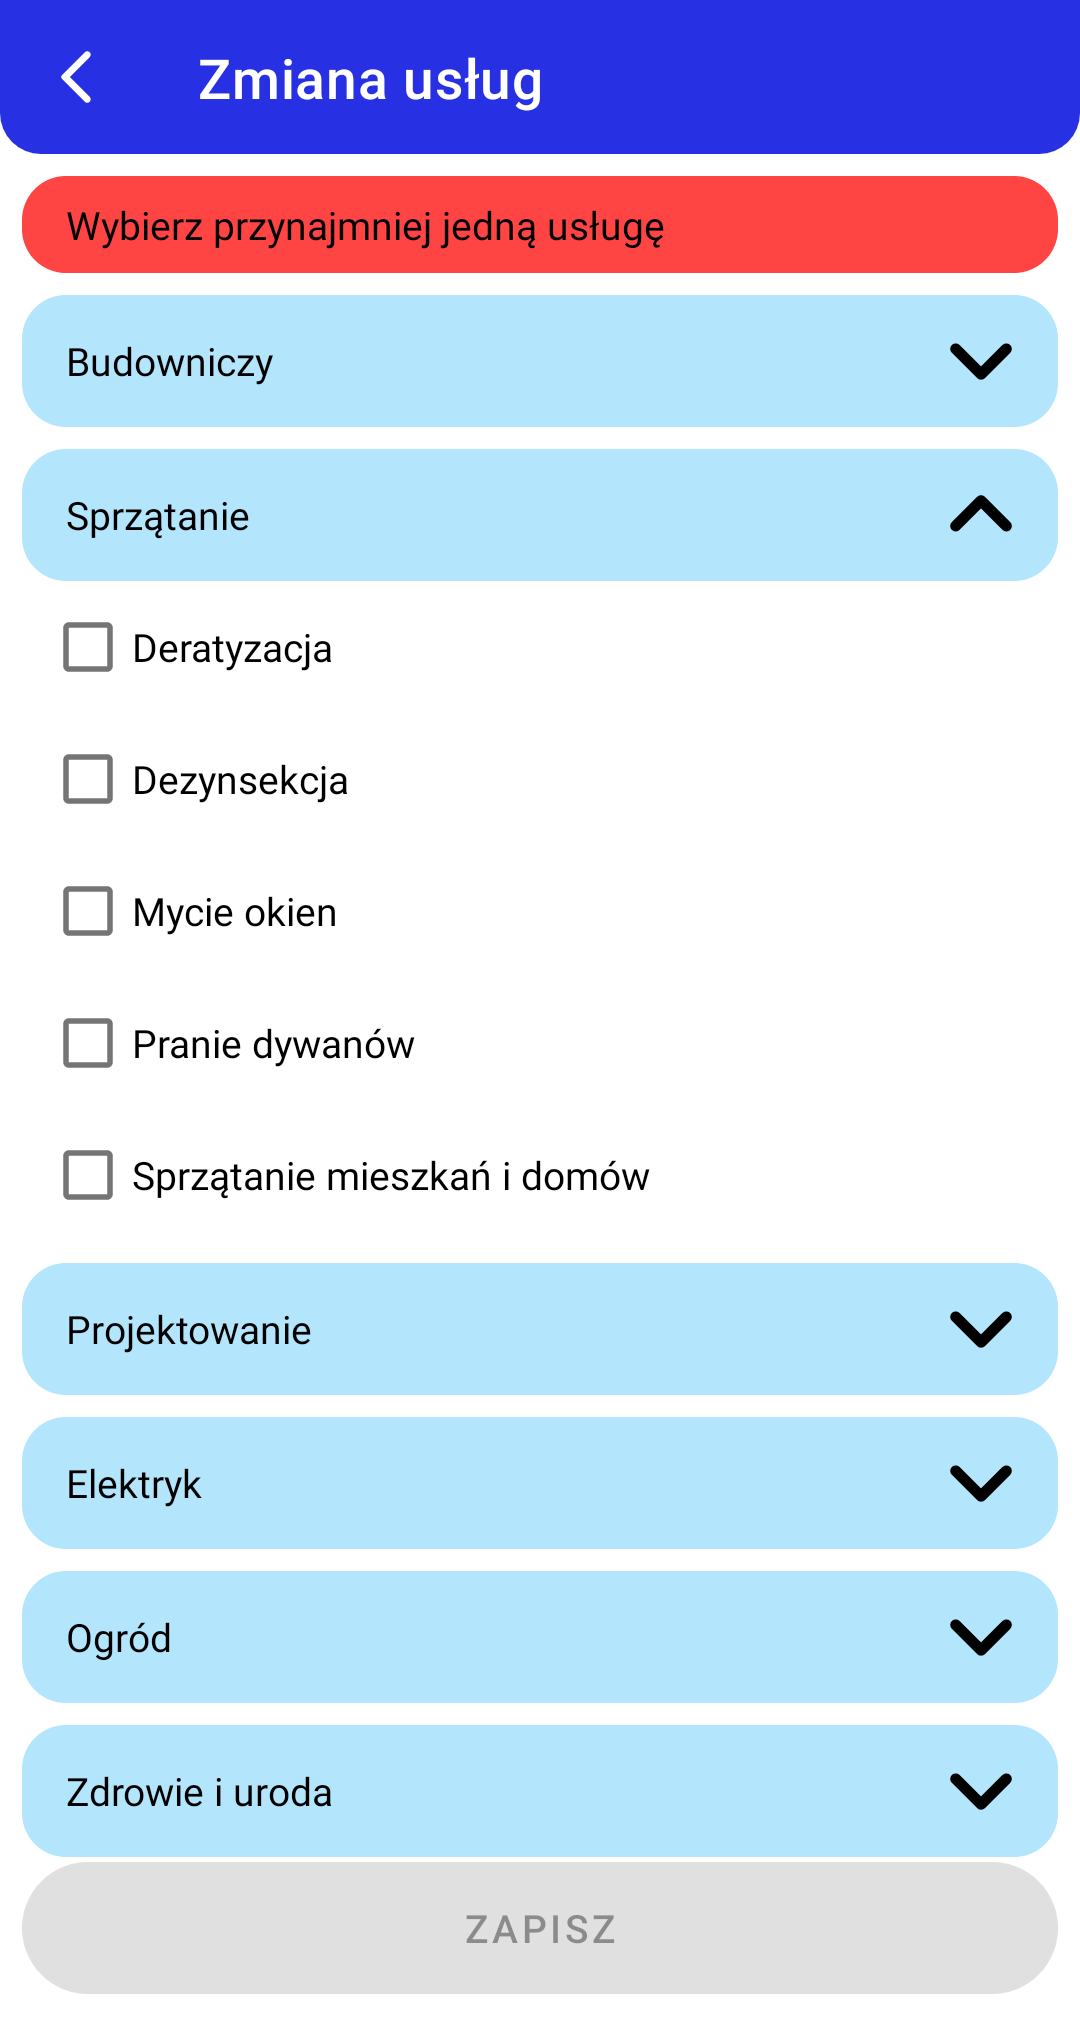
\includegraphics[width=0.33\linewidth]{screens/services.png}}
  \caption{Ekran zmiany świadczonych usług}
  \label{fig:services}
\end{figure}
